\documentclass[conference]{IEEEtran} % default font size: 10pt
\usepackage{times,microtype}

\usepackage{graphicx}
\usepackage[caption=false]{subfig}
\graphicspath{{images/}}

\usepackage{amsmath,amssymb,mathtools}

\renewcommand{\vec}[1]{\boldsymbol{#1}}
\DeclarePairedDelimiter{\abs}{\lvert}{\rvert}
\DeclarePairedDelimiter{\norm}{\lVert}{\rVert}
%
%\usepackage{lipsum,xcolor} % TODO: remove once fully written

% numbers option provides compact numerical references in the text.
\usepackage[numbers]{natbib}
\usepackage{multicol}
\usepackage[bookmarks=true]{hyperref}

\pdfinfo{ % TODO: update info below
   /Author (Homer Simpson)
   /Title  (Robots: Our new overlords)
   % /CreationDate (D:20101201120000)
   /Subject (Robots)
   /Keywords (Robots;Overlords)
}

\begin{document}

% TODO: paper title
\title{Is minimalistic MPC based on centroidal dynamics enough to race complex vehicles?}

% You will get a Paper-ID when submitting a pdf file to the conference system TODO: update info below
\author{Author Names Omitted. Paper-ID [add your ID here]}

%\author{\authorblockN{Michael Shell}
%\authorblockA{School of Electrical and\\Computer Engineering\\
%Georgia Institute of Technology\\
%Atlanta, Georgia 30332--0250\\
%Email: mshell@ece.gatech.edu}
%\and
%\authorblockN{Homer Simpson}
%\authorblockA{Twentieth Century Fox\\
%Springfield, USA\\
%Email: homer@thesimpsons.com}
%\and
%\authorblockN{James Kirk\\ and Montgomery Scott}
%\authorblockA{Starfleet Academy\\
%San Francisco, California 96678-2391\\
%Telephone: (800) 555--1212\\
%Fax: (888) 555--1212}}


% avoiding spaces at the end of the author lines is not a problem with
% conference papers because we don't use \thanks or \IEEEmembership


% for over three affiliations, or if they all won't fit within the width
% of the page, use this alternative format:
%
%\author{\authorblockN{Michael Shell\authorrefmark{1},
%Homer Simpson\authorrefmark{2},
%James Kirk\authorrefmark{3},
%Montgomery Scott\authorrefmark{3} and
%Eldon Tyrell\authorrefmark{4}}
%\authorblockA{\authorrefmark{1}School of Electrical and Computer Engineering\\
%Georgia Institute of Technology,
%Atlanta, Georgia 30332--0250\\ Email: mshell@ece.gatech.edu}
%\authorblockA{\authorrefmark{2}Twentieth Century Fox, Springfield, USA\\
%Email: homer@thesimpsons.com}
%\authorblockA{\authorrefmark{3}Starfleet Academy, San Francisco, California 96678-2391\\
%Telephone: (800) 555--1212, Fax: (888) 555--1212}
%\authorblockA{\authorrefmark{4}Tyrell Inc., 123 Replicant Street, Los Angeles, California 90210--4321}}


\maketitle

% ----------------------------------------------------------------------------------------

\begin{abstract}
MPC online control problem enhanced in CasADi, a framework written by \citet{Andersson2019}.
\end{abstract}

\IEEEpeerreviewmaketitle

\section{Introduction}

%\textcolor{gray}{\lipsum[1]}

% ----------------------------------------------------------------------------------------

\section{Proposed approach} % TODO: if the method has a name, use it here as section title

%\textcolor{gray}{\lipsum[2]}

\subsection{Vehicle model}

%\textcolor{gray}{\lipsum[3]}
\subsection{MPC Model}
In order to build an MPC internal model with its own dynamics, and which is as simple as possible, a point mass model is chosen.
This model has 3 DOF and encloses in itself the fundamental parameters of the driven vehicle as mass, aerodynamic coefficients, grip and power limits for braking and traction phases.
With this MPC internal model, the optimal control problem is formulated in order to find the optimal control sequence necessary to minimize the travel time of the next N meters of the track. In particular the control inputs of the point mass model are the total longitudinal force $F_{x}$, and the angular acceleration along the $z$-axes $r_p = dr/dt$, where $r$ is the yaw rate.
The point mass model dynamics is then formulated in spatial domain instead of the time one, and the \textit{direct collocation} is used to transform the OCP into an NLP. The NLP is coded in a scripting environment using the Matlab interface to the open-source CasADi framework~\cite{Andersson2019}, which provides building
blocks to efficiently formulate and solve large-scale optimization problems, and solved through IPOPT \textbf{cita ipopt}.

Once the problem is solved an optimal control sequence for the steering angle has to be extracted from the NLP solution. In order to do that we use the following formula
\begin{equation}
\delta = \alpha_{1} + \beta_1 = F_{y_{11}}/C_\alpha + (v + ra_1)/u
\end{equation}
where the notation is based on \textbf{cita Guiggiani}, hence $C_\alpha$ is the cornering stiffness of the front tire, $a_1$ is the distance between the CoM and the front axle, and we assume that the tire slip angles and the vehicle slip angles are equal for the wheels of the same axle, hence $\alpha_{11} = \alpha_{12} = \alpha_{1}$ and  $\beta_{11} = \beta_{12} = \beta_{1}$.
Furthermore, the lateral force of the front wheels are extimated with a steady state assumption in a way that $F_{y_{11}} = F_{y_{12}} = F_{y}a_2/(2l)$, where $F_{y}$ is the total lateral force acting on the point mass model, available from the NLP solution, $a_2$ is the distance between the CoM and the rear axle and $l$ is the wheelbase.



For what concern the race track, it is assumed planar and modelled through the parametric 2D curve
\begin{equation}
\mathcal C(\alpha) = \{ \vec x (\alpha) = [x(\alpha), y(\alpha)]^T \in \mathbb{R}^2 : \alpha \in [\alpha_0, \alpha_f] \}
\end{equation}
%
that identifies the road centerline, and the 1D curve $\mathcal W(\alpha)$ that specifies the track width.
With reference to Figure~\ref{fig:scheme_frenet_serret_refsys}, the \emph{curve parameter} $\alpha$ uniquely selects a point $\vec F = \vec x(\alpha)$ that defines the origin of the \emph{Frenet-Serret frame} $\mathcal F = \{ \vec F, (\vec t, \vec p) \}$ whose unit vectors are, respectively, the tangent $\vec t$ and the normal $\vec p$ of the curve $\mathcal C$ in the point $\vec F$.
%
The vehicle reference system $\mathcal V = \{ \vec G, (\vec i, \vec j) \}$ can be expressed in terms of the moving frame $\mathcal F$ with a \emph{lateral displacement} $e_p$ along the track normal direction $\vec p$ and the \emph{heading error} $e_\psi$.
% = \psi_f - \psi_v
In order to maintain $\mathcal F$ side-by-side with $\mathcal V$, the Frenet-Serret system has to proceed together with the vehicle: this leads to a relation between vehicle and Frenet-Serret velocities that ultimately imposes a bound between time and $\alpha$ increments.

%The final formulation of the vehicle model dynamics, % TODO: ref to standard formulation, if previously exposed
%extended with lateral displacement, heading error and transposed in spatial domain is
%
%\begin{equation} \left\{
%\begin{aligned}
%u_{,\alpha} &= \frac{\norm{\hat{\vec x}_{,\alpha}}}{s_p} \left[ \frac{1}{m} (F_{x} - X_a) + vr \right] \\
%v_{,\alpha} &= \frac{\norm{\hat{\vec x}_{,\alpha}}}{s_p} \left[ \frac{F_{y}}{m} - ur \right] \\
%r_{,\alpha} &= \frac{\norm{\hat{\vec x}_{,\alpha}}}{s_p} r_{p}  \\
%e_{p,\alpha} &= \frac{\norm{\hat{\vec x}_{,\alpha}}}{s_p} \left[ u \sin{e_\psi} + v \cos{e_\psi} \right] \\
%e_{\psi,\alpha} &= \norm{\hat{\vec x}_{,\alpha}} \left( \frac{r}{s_p} - k \right),
%\end{aligned} \right.
%\label{eq:vehicle_state_update_alpha_domain}
%\end{equation}
%%
%where the notation $u_{,\alpha} = \frac{du}{d \alpha}$ has been used to shorten derivative notations.

\begin{figure}[htb] \centering
	%  \subfloat[]
	%    {\includegraphics[width=.5\linewidth]{example-image-a}} % NOTE: this needs `mwe' package
	%  \quad
	\subfloat[]{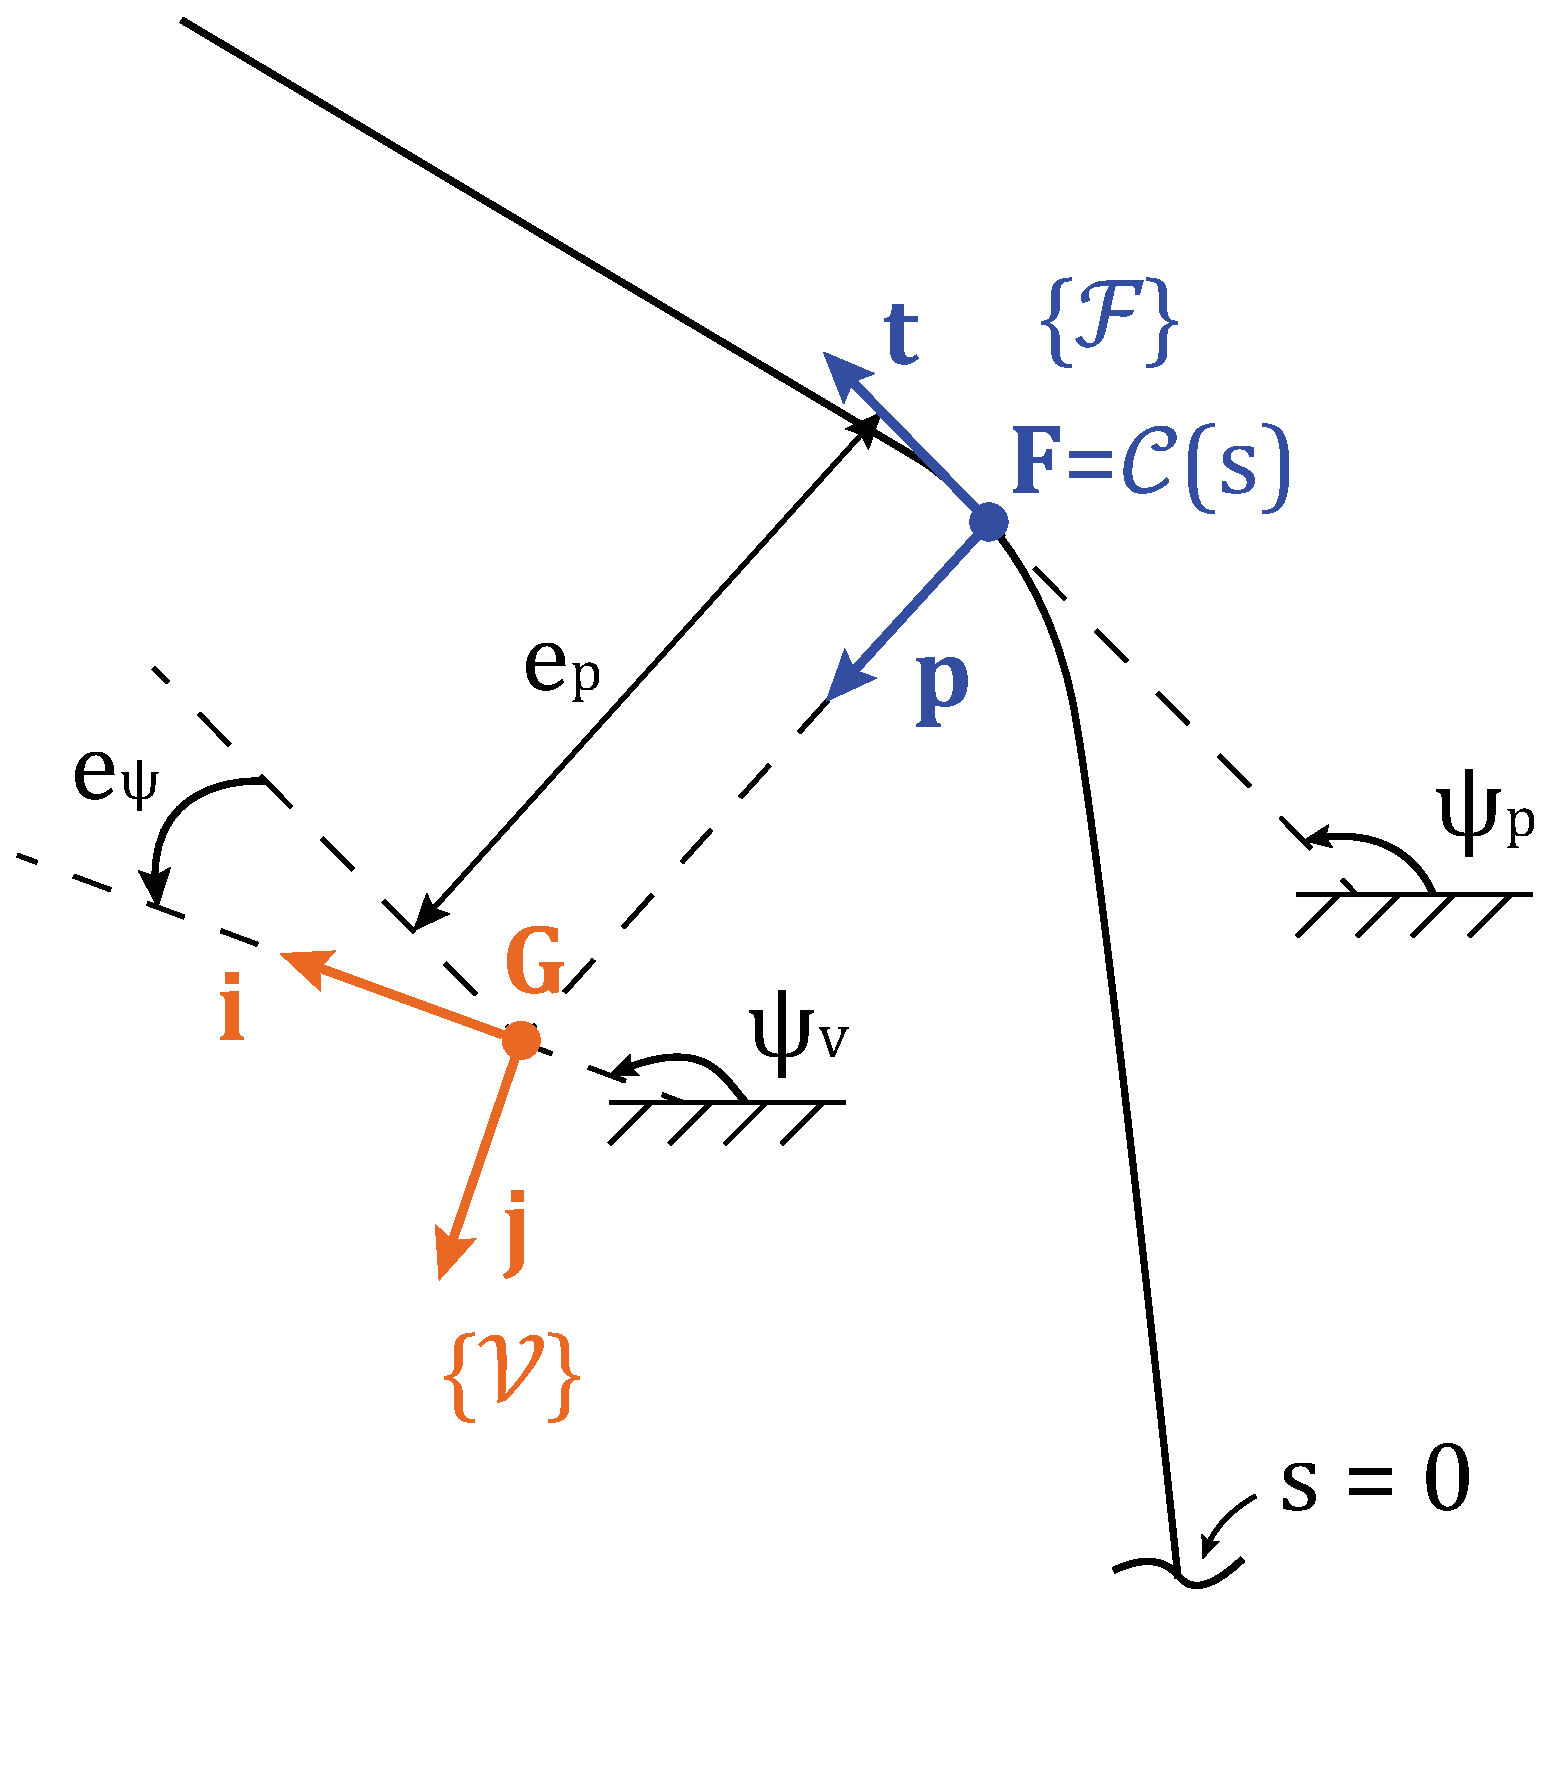
\includegraphics[width=.4\linewidth]{scheme_frenet_serret_refsys}
		\label{fig:scheme_frenet_serret_refsys}}
	\caption{(\textbf{a}) vehicle pose respect to the Frenet-Serret reference system identified on the track curve.}
	\label{fig:scheme_frenet_serret}
\end{figure}

\subsection{Offset-free MPC}






% \subsection{OCP problem formulation}

% The Optimal Control Problem (OCP) is



%\textcolor{gray}{\lipsum[4]}

% ----------------------------------------------------------------------------------------

\section{Preliminary results}
The MPC controller is tested on Indianapolis oval track racing. In particular, three different simulation are performed: (i) lap-time simulation with MPC controller, (ii) lap-time simulation with MPC controller in which the aerodynamic drag is removed from the model equations, (iii) lap-time simulation with offset-free MPC, where the aerodynamic drag is estimated through the technique explained in \textbf{cita sez. offset-free}.

The solutions in terms of trajectories of the real vehicle and controls input provided to it, are shown below, for the entry phase of the first curve. 

\begin{figure}[htb] \centering
    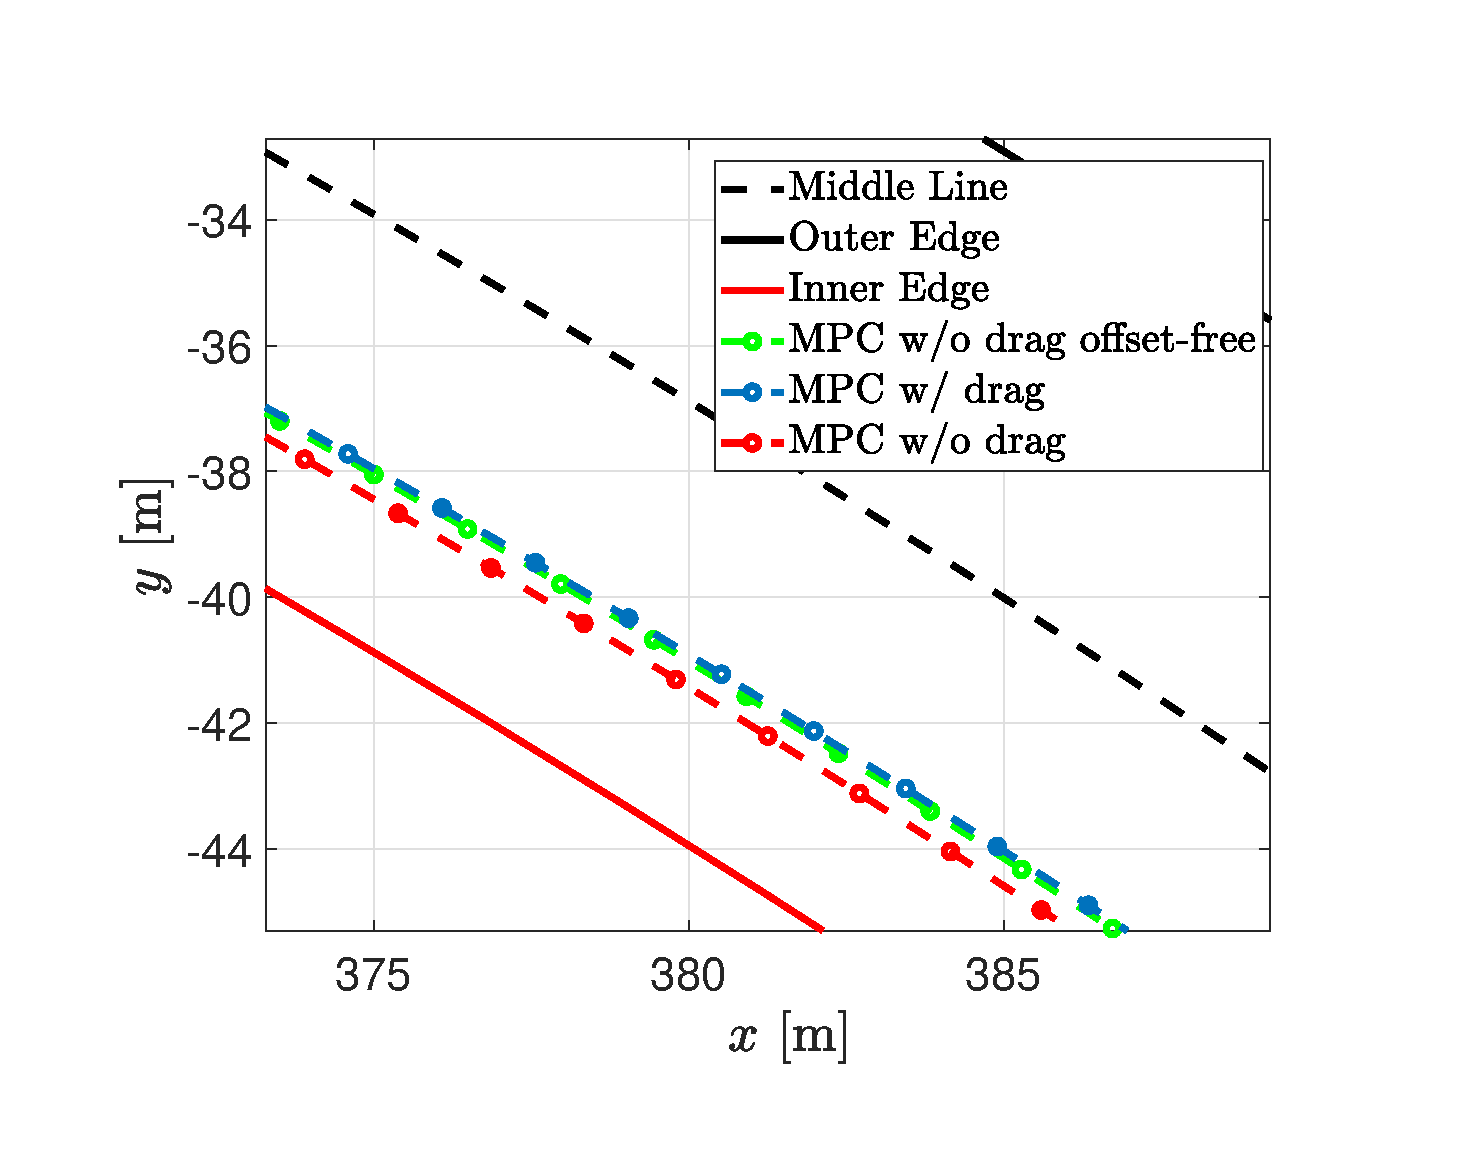
\includegraphics[width=1.\linewidth]{Trajectories2}
	\caption{Trajectories comparison between lap simulation with MPC (blue), MPC offset-free (green), MPC without drag (red)}
	\label{fig:Trajectories2}
\end{figure}

\begin{figure}[htb] \centering
	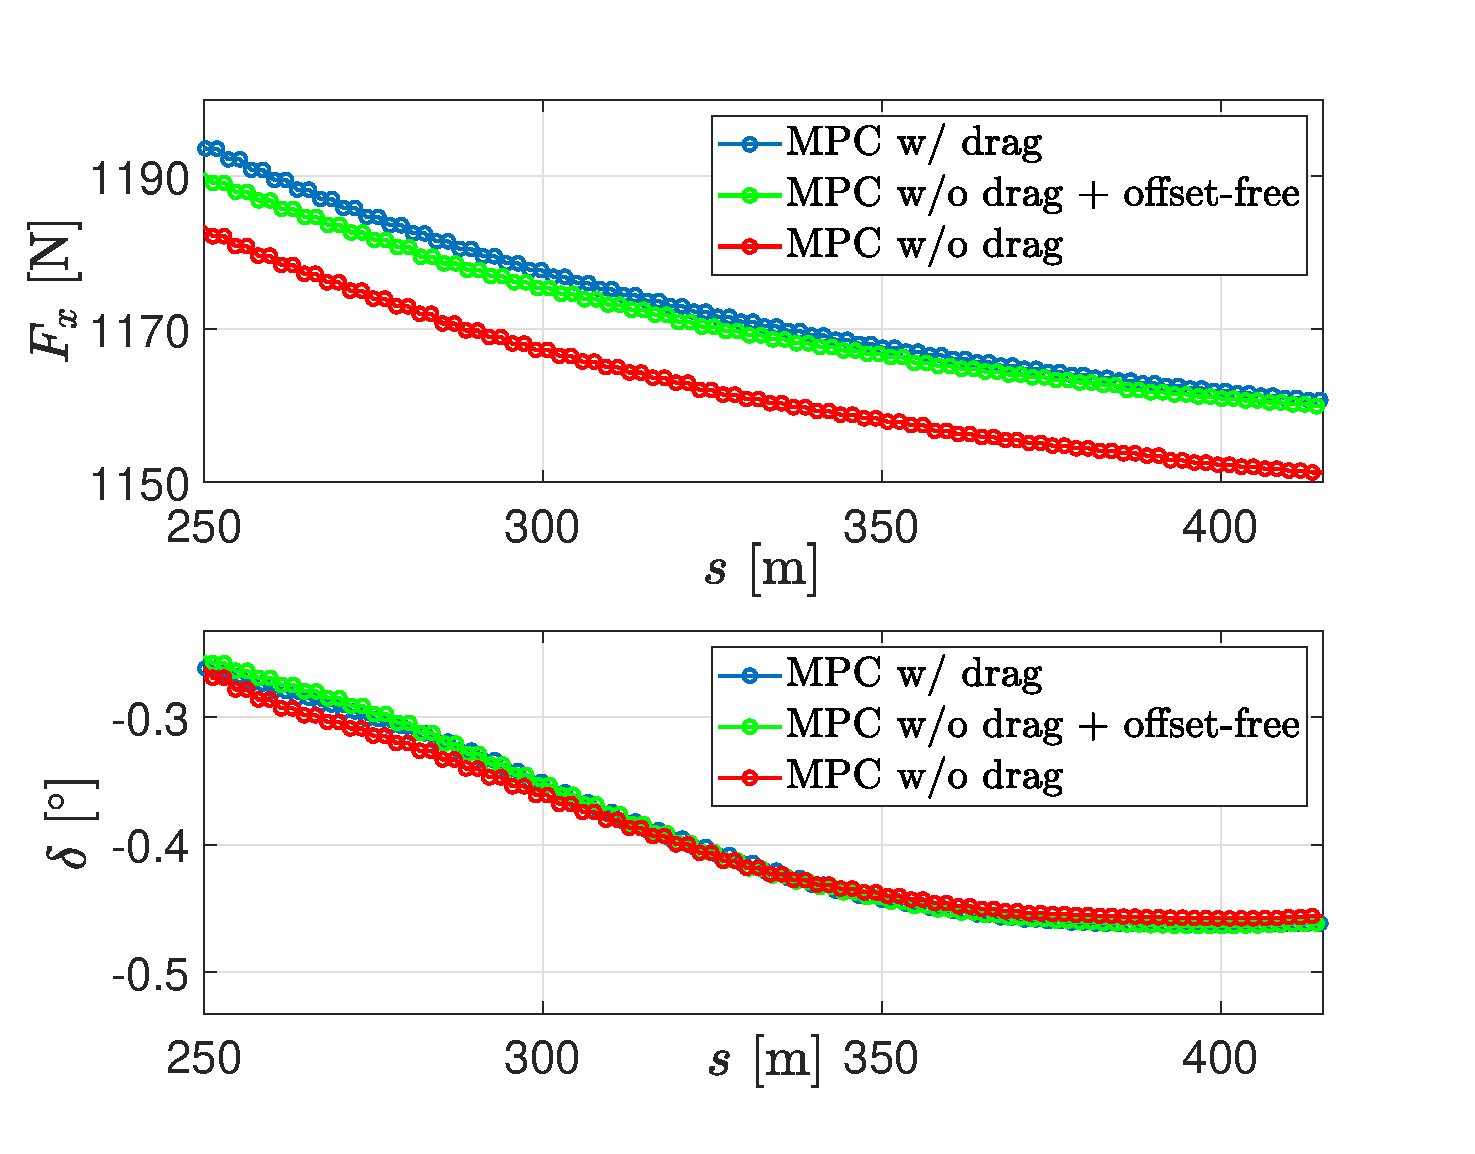
\includegraphics[width=1.\linewidth]{steer_fx}
	\caption{Comparison between control inputs, longitudinal force (top), steering angle of the front wheel (bottom), obtained with MPC (blue), MPC offset-free (green) and MPC without drag (red)}
	\label{fig:steer_fx}
\end{figure}

Figures.\ref{fig:Trajectories2} - \ref{fig:steer_fx} highlight how MPC with drag and MPC offset-free are able to drive the Adams vehicle in the same way, with a lap-time difference of $6.5$ms. Instead if the aerodynamic drag is not modeled inside the MPC, the controller is not able to maintain the real vehicle on the track, in fact the simulation failed on the entry phase of the second curve.

%\textcolor{gray}{\lipsum[5]}

% ----------------------------------------------------------------------------------------

\section{Conclusion}
The minimalistic MPC based on a point mass model with its body-fixed reference system is enough to race complex vehicle. In particular the parameters of the MPC model as the mass, the aerodynamic coefficients or power limits, have to be equal to those of the driven car. In this way we can consider the point mass model as a condensed model of the complex vehicle.

Furthermore, the offset-free technique is an helpful and efficient method in order to modeled in a simple way some fundamental characteristics of the complex vehicle. As an example we consider not knowing the aerodynamic drag coefficient and we estimate drag force with the disturbance $d$.

As a future developments of this work, some modifies to the MPC internal model, as a new approach to extract the steer angle, has to be found in order to drive the complex car on its limits. 
\label{sec:conclusion}

%\textcolor{gray}{\lipsum[6]}

% ----------------------------------------------------------------------------------------

%% Use plainnat to work nicely with natbib.
\bibliographystyle{plainnat}
\bibliography{references}

\end{document} 